Out of the 16 weekly meetings throughout a semester, 13 present new topics.
By the end of the second week generalised coordinates were used to calculate the mechanical energy of various systems with ad-hoc Sympy-based functions provided by the teaching staff.
From third to fifth week the Euler-Lagrange approach is implemented into code to simulate the dynamics of multiple point mass systems.
By the eighth week, constrained forces and non-conservative ones are calculated.
Starting at the ninth week the course focus on extended bodies modelled as rigid bodies employing inertia tensors and Euler equations for rotation.
The final weeks are devoted to vibrations including forced harmonic oscillations and modal analysis at systems with multiple degrees of freedom.
Further details beyond this brief description of the weekly topics can be obtained from the full schedule available at the course repository \cite{repositorio-victor}.
The progression of the course is illustrated by the following selection of some of these topics.


\textbf{Week 1: vector kinematics}
After a brief introduction to the flipped classroom methodology and description of the coding tools to use, a hand-on practice on the use of Google Colab begins.
As a first exposure to Sympy calculus capabilities, students are presented with a review of vector kinematics with code for time-differention of position vector in some reference frames and coordinate systems as shown in figure \ref{fig:week1_differentiation}.

\begin{figure}[!ht]
    \centering
    \includegraphics[width=0.95\linewidth]{figuras/week1_differentiation.png}
    \caption{The first lesson in Jupyter notebooks: a review of kinematics where Sympy calculus functions are used.}
    \label{fig:week1_differentiation}
\end{figure}

Then in a second lesson notebook the construction of a function to calculate the kinetic energy for a compound pendulum is explained step-wise. 
Students are encouraged to review the \LaTeX\ notation used in that notebook.


\textbf{Week 3: Euler-Lagrange formalism}
This is the main tool of analytical mechanics that students will instrumentalise to generate diffential equations to describe, at this stage of the course, the dynamics of multiple point mass systems.
After a step-wise construction, akin that followed with functions for energies, a function to generate these equations is provided to the student in an example problem as illustrated by figure \ref{fig:week4_eulerLagrangeFunction}.
This code will be re-used by the student from now on through the course to address problems at every exercises set.

\begin{figure}[ht]
    \centering
    \includegraphics[width=\linewidth]{figuras/week4_eulerLagrangeFunction.png}
    \caption{The Euler-Lagrange formalism is the center piece of the analytical tools used in the course. After a step by step construction, a fully assembled function would allow to apply it in code used thereafter.}
    \label{fig:week4_eulerLagrangeFunction}
\end{figure}


So far, code has been used to perform the same steps that are solved on a blackboard or paper in a conventional rational mechanics course to arrive at differential equations that are only solved for trivial cases.
In contrast, using Sympy quickly solves complex systems for acceleration a function of generalized coordinates and velocities as shown in Figure \ref{fig:clase4ac}.
Performing such a task manually would require a non-negligible amount of time and effort even for this system with only two degrees of freedom.

\begin{figure}[!ht]
\centering
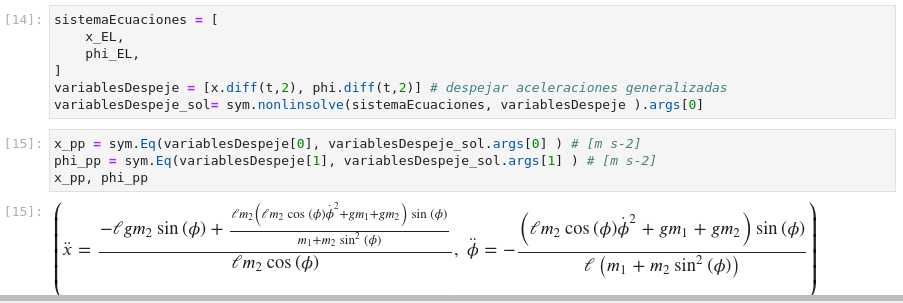
\includegraphics[width=\linewidth]{figuras/clase4Aceleraciones.png}
\caption{The resolution of systems of differential equations of certain complexity is avoided in conventional courses. In this course, it only takes a couple of lines of code with functions in the Sympy library.}
\label{fig:clase4ac}
\end{figure}



\textbf{Week 5: simulation}
Students passed a numerical analysis course to enroll in this course where such knowledge will be used.
In this lesson, the fundamentals of numerical resolution methods for differential equations are reviewed and how they would be implemented in a state vector notation suitable for efficient processing.
Immediately after the review of fundamentals, the functions of the scientific calculation library Scipy are shown in action to efficiently obtain solutions for the dynamics of a two-degrees-of-freedom system as illustrated by Figure \ref{fig:clase5sol}.

\begin{figure}[!ht]
\centering
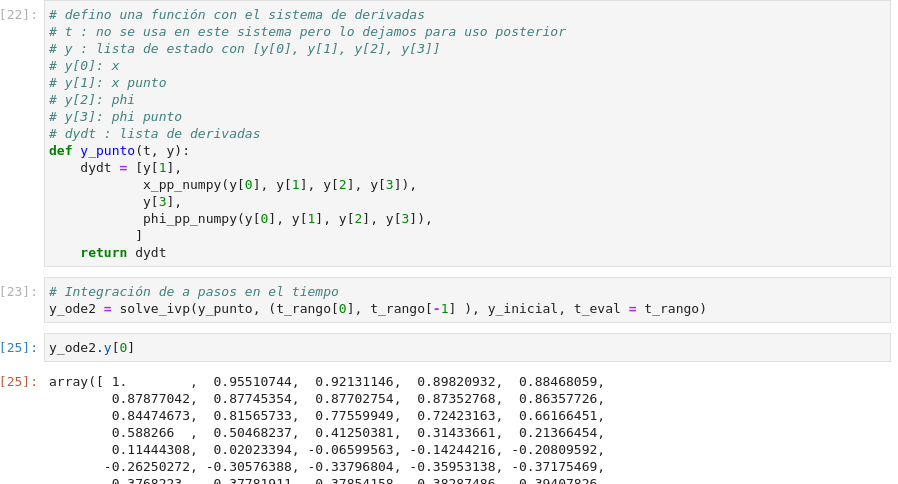
\includegraphics[width=\linewidth]{figuras/clase5Soluciones.png}
\caption{The system of equations for the dynamics of a two-degrees-of-freedom system is numerically solved with functions of the SciPy library.}
\label{fig:clase5sol}
\end{figure}

Generalized positions and velocities obtained numerically at times of interest are graphically represented, as shown by figure \ref{fig:clase5rep}, which is useful to discuss students whether the behavior of the system is consistent with what can be predicted from a qualitative analysis of this simple system.
Confirming that the symbolic and numerical calculation tools used obtain correct results gives confidence in them in view of applying this tools to more complex systems.

\begin{figure}[!ht]
	\centering
	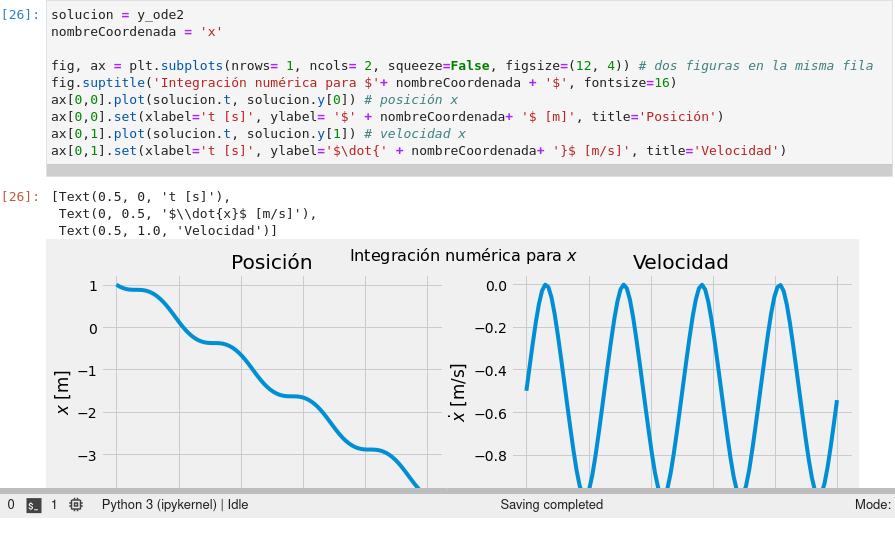
\includegraphics[width=\linewidth]{figuras/clase5Representación.png}
	\caption{
		Visualisation of results obtained by numerical calculations.
		Corroborating that what is represented corresponds to a qualitative analysis of the dynamics of the system creates confidence in the students in this tool.
	}
	\label{fig:clase5rep}
\end{figure}

\textbf{Final weeks.}
Towards the end of our course the students of our course have already developed the ability to autonomously analyse ``realistic'' systems resembling mechanical devices found in the industry.
To present them a challenge in this line, they are assigned a final project in which they must calculate the torques required for the motors of a highly simplified industrial robotic arm to perform a sequence of movements. 
Examples of the results of students' work in response to this proposal are shown in figure \ref{fig:robotarm}.

\begin{figure}[!ht]
\centering
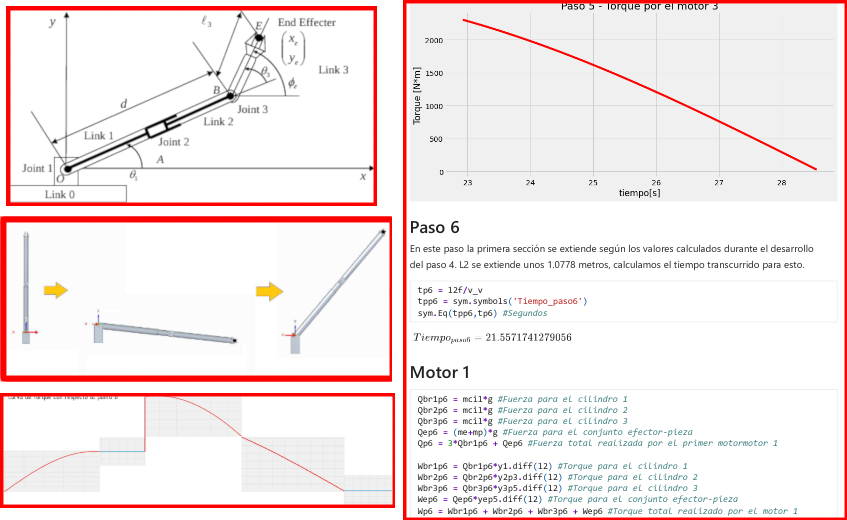
\includegraphics[width=\linewidth]{figuras/robotArm.png}
\caption{To be able to perform even a simple movement, motors of an industrial arm  must apply a sequence of torques. Students calculate them in a final assignment that reflects their mastery of analytical and computer tools taught at the course.}
\label{fig:robotarm}
\end{figure}

Students are required to present their results in an oral presentation to the teaching staff.
With this we aim to push them to improve their conmunication skills, not only by writting their work in an ordely fashion, but also to prepare a speech to defend it, a stressful situation but a must for any business-like setting.
